\documentclass[review]{elsarticle}
\usepackage{hyperref,lineno}
\usepackage{wrapfig}
\usepackage{lscape}
\usepackage{rotating}
\usepackage{xcolor}
\usepackage[utf8]{inputenc}
\modulolinenumbers[5]


\newcommand{\memo}[2]{\textcolor{#1}{#2}}
\newcommand{\maria}[1]{\memo{red}{#1\\}}
\newcommand{\xavi}[1]{\memo{magenta}{XRC: #1\\}}

%\journal{Journal of Archaeological Science}


\bibliographystyle{model2-names.bst}\biboptions{authoryear}


\begin{document}

\begin{frontmatter}

\title{The markings of the trade: exploring the patterns of olive oil production in Roman Baetica}

\author[ceipacadress]{Maria Coto-Sarmiento\corref{mycorrespondingauthor}}
\cortext[mycorrespondingauthor]{Corresponding author}
\ead{mcotsar@gmail.com}


\author[edadress]{Xavier Rubio-Campillo}

\address[edadress]{School of History, Classic \& Archaeology, Room OOM.33, William Robertson Wing, Old Medical School, Teviot Place, University of Edinburgh, UK}
\address[ceipacadress]{CEIPAC, Department of Prehistory and Archaeology, Montalegre, 6-8, 08001, University of Barcelona, Barcelona, Spain}

\begin{keyword}
Roman Empire; amphora workshops; Dressel 20; social learning; cultural evolution
\end{keyword}


\begin{abstract}

The aim of this study is to explore economics dynamics in the production and distribution of olive oil trade. 
Our case of study has been focused on the production processes located in \textit{Baetica} province (currently Andalusia) from 1st to 3rd AD. In particular, we want to detect patterns of olive oil production that link amphora workshops and amphoric stamps. \textit{Baetica} became important production and distribution centre during the Roman Empire. However, it remains under debate about how this province was organised and whether it could be possible to identify patterns in the olive oil market. Amphoric stamps are used to identify the presence of different groups that might share similar stamps. To achieve this goal, we analyse a set of stamps from two centres: 1) producer centres by analysing different workshops in \textit{Baetica} province and 2) two Roman provinces such as \textit{Germania} and \textit{Britannia} as a receptor centres. They will be used to detect a connection between the distribution of amphoric stamps and the economic structure in both centres. Here we use methods borrowed from Ecology that allow us to identify if amphora workshops share similar amphoric stamps depending on the spatial distance. 

The analysis explores how the quantitative approach provides a useful tool for the interpretation of the economic processes. Finally, results pretend to highlight the organisation of Baetican olive oil production in the Roman Empire linked to the differences observed in the archaeological evidence.

\end{abstract}


\end{frontmatter}


\section{Introduction}


%\xavi{queda raro esto de "en arqueología la cultura material nos permite ver la distribución en el Mediterráneo". Yo iría directa a hablar del Mediterráneo sin la primera frase.}


The role of the Mediterranean sea for the trade had an enormous impact during the Roman Empire. The spread of thousands of different goods along maritime shipping allowed a progressive exploitation of communication networks and a major interaction between communities \citep{rodriguez_baetican_1998, 
temin_market_2001,
bevan_mediterranean_2014}. The exchange of different products between regions can be seen in both archaeological and written records as a frequent indicator of Roman trade.  

%Material culture is one of the most frequent indicators of trade in the archaeological record. In archaeology, they allow us to highlight a part of the mechanism of production and distribution of goods along the Mediterranean \citep{bevan_mediterranean_2014}. Particularly, the spread of these factors had an important impact during the Roman Age, when the progressive exploitation of communication networks allowed a major interaction between communities \citep{orengo_seeds_2016}\xavi{aquí faltan citas de obras más generales; esto es un ejemplo pero muy específico no?}. 
%spread of goods and ideas had a enormous impact during the Roman Empire. The progressive exploitation of communication networks allowed a major interaction between communities
%This can be seen by the fact that material culture is found in different regions along the Mediterranean as a frequent indicator of trade exchange in the archaeological record. 

Given this fact, an important mechanism of production control under the Roman government was created spreading by different areas attending to the richness of different places. Roman provinces such as \textit{Baetica} (currently Andalusia, south Spain) became important production centres of olive oil during the Roman Empire. Olive oil was considered the liquid gold since it was used in different aspect of daily life for cooking, hygiene or lighting  \citep{mattingly_d.j._oil_1988}. As a consequence, this product was distributed in a large number of amphorae along the provinces, mostly to supply the Roman Army and Italy \citep{blazquez_exportacion_1980}. 


The understanding of the olive oil production processes has been widely discussed over many decades\citep{rodriguez_economioleicola_1977, Chic_hispania_1997,millet_anforas_1998}. Despite this topic remains under debate: what patterns were followed for the distribution of olive oil to the different provinces?
Did each province follow a different pattern for its distribution? Nor the lack of written records has made possible to detect any indication of patterns in the olive oil market.

Advances in the research of the Roman world have currently led an environment with more diverse commercial dynamics \citep{duncan1982economy,
temin_economy_2006,
quantifyingwilson2009}. The application of different quantitative approaches combined with the archaeological evidence has allowed us partly to deal with the complexity of the Roman production \citep{brughmans_roman_2016,
orengo_seeds_2016,bayesian_2018,
coto-sarmiento_identifying_2018,
rubio-campillo_ecology_2018}.


%\xavi{este aim es demasiado general}
%This paper aims to understand the production dynamics in connection with different areas within the Roman Empire. 
This paper aims to study the olive oil market connection between province by calculating the similarity index. Specifically, our work pretends to detect microeconomic processes focused on a commercial product from a specific province \citep{isaksen_network_2006}. We want to understand the pattern of olive oil production linked to amphora workshops and amphoric stamps used to mark them. We focus here on exploring the economic relation between stamps and amphora production and distribution centres. 

Two case studies have been studied in order to analyse the relation between production centres (\textit{Baetica}) and consumption centres (\textit{Britannia} and \textit{Germania}). In the case of \textit{Baetica} province, we want to identify the role of the stamps in the organisation of the workshop; in Roman provinces, our aim is detecting groups of stamps concentrated in an area or if some groups have an important role for the exportation of olive oil in those provinces. This economic connection could be identified by different aspects: a) correlation between spatial distance and centres based on the idea that closer workshops concentrate similar amphoric stamps in a specific area than the distant workshops and b) groups of similar stamps were concentrated in a specific Roman province. 
%\xavi{affected? No sería "identified"? Es decir, la correlación es la evidencia, pero la causa sería la interacción económica...no?}

%Our case study examines the relationship between the distribution of amphoric stamps and the workshops.
In particular, we study the distribution of amphoric stamp in order to identify a correlation between geographical distance and amphoric stamps. Based on this assumption, we proposed three hypotheses: a) we can identify a correlation between spatial distance and the distribution of stamps, b) stamps located in close workshops share similar traits and c) Low mobility of amphoric stamps to other regions: stamps always stay in the same region.  


To do this, a population approach has been used to analyse the dispersion of stamps between amphora workshops \citep{rubio-campillo_ecology_2018}. Stamps will be used to identify economic patterns by analysing their similarity. If workshops and provinces share stamps with similar traits, then we can identify connections. By contrast, if we do not detect similar stamps between workshops, then workshops worked independently. 

%\xavi{esta frase tendría que ir al final de la Intro; si pones subsecciones entonces queda muy raro creo}

The paper addresses these questions as follows: the next section introduces the historical context. Section two displays the dataset and the methods used for the analysis. Section three presents the results and the last section shows the discussion and the main conclusions of this work. 
 
%\xavi{creo que le falta chicha aquí, sobre qué se ha hecho hasta ahora, qué quieres saber específicamente, el caso de estudio...}


\section{The Amphoric production in Baetica province}


The high demand of Roman provinces stimulated by the good condition of the \textit{Baetica} lands allowed to develop a massive infrastructure of olive oil production. The production and distribution of olive oil were growing exponentially for almost three centuries \citep{remesal_concierto}. As a result, hundreds of amphora workshops were made to support this high demand of the Roman Empire. The amphora workshops were situated in different locations in \textit{Baetica} province, along the rivers Guadalquivir and Genil (see Fig.\ref{workshop}).

The location of the workshops with a riverine connectivity allowed to set up a connection with the Mediterranean and Atlantic routes \citep{garcia_vargas_enrique_formal_2010}.

\begin{figure}[htp]
	\centering
\includegraphics[width=\linewidth]{figs/workshop1}
\caption{Distribution of the workshops in Baetica province}
\label{workshop}
\end{figure} 

%\xavi{Yo aplicaría aquí el feedback de los mapas para lo del libro...no creo que colorearlo basándose en el DEM aporte demasiado no?}

The chronology in the workshops is widely diverse from the first to the third centuries AD \citep{millet_anforas_1998,rodriguez_baetican_1998,chic2005comercio}. 

The majority of olive oil amphorae produced in this province and shipped through the provinces belong to Dressel 20 type \citep{dressel_ricerche_1878,
millet_anforas_1998}. This amphora is commonly associated with the transportation of Baetican olive oil during the Roman Empire \citep{berni_millet_epigrafianforica_2008}. Most Dressel 20 were marked in stamps, inked in \textit{tituli picti} and incise in \textit{graffiti} with different information still unknown. Indeed, most of the inscriptions on the amphora have not enough analysed due to the fragmentation of the material or the shortage of samples \citep{aguilera_evolucion_2007,rovira_guardiola_grafitos_2007}. 


Some stamps show a more specific chronology while the majority of them display a large activity of production that it can be difficult for specifying an accurate chronology. This could be due to two reasons; firstly, most of the workshops were partially excavated and focused on archaeological surveys in order to collect the maximum stamps as possible; secondly, Dressel 20 was produced during almost three centuries with apparently few changes \citep{berni_piero_chapter_2017}.

\section{Britannia and Germania}

%\xavi{Esta parte más histórica está chachi pero creo que debería estar en la Intro. Ahí podrías explicar la organización, y a partir de estas fuentes escritas plantear preguntas e hipótesis que justifiquen el paper y tu análisis usando arqueología.}


The conquest of new provinces allowed to the Roman Empire the arrival of new resources. This lead to a progressive change in the economic and social structure. As a result, Augusto's administration created the figure of the \textit{praefectura annonae} for the supply of wheat. The role of the \textit{praefectura annonae} was mainly to provide though \textit{frumentationes} a quantity per month of wheat to Roman citizens \citep{remesal_annona_1986,remesal_concierto}. 


The consumption of olive oil in \textit{Britannia} was residual until starting the Roman conquest \citep{funari_corpus_1996,
carreras_abastecimiento_2003}.

It is well known that this product was not frequently consumed by indigenous population. The absence of olive oil importation before the conquest can be reflected by the shortage of this product until the arrival of a high percentage of Dressel 20 amphorae to \textit{Britannia} \citep[ 1]{carreras_britannia_1998}. Additionally, the land of \textit{Britannia} showed inadequate for the olive oil production due to low environmental conditions. This issue was necessary for creating an important export apparatus from \textit{Baetica} to supply Roman army.

At this moment, we detect an increase of the olive oil exportation concurring with the displacement of legions during the military campaigns \citep[161]{monfort_britanniaen_1998}. This fact will be spatial incidence in sites close at Hadrian Wall.  
Olive oil production in \textit{Baetica} would cross the Atlantic until they reached the province and redistribute throughout the area from a series of strategic points \citep{carreras_atlantic_2012}. The increase of the exportation of Dressel 20 amphorae created an important commercial network for exchanges. Thus, the network was mainly focused on the support of soldiers during the military campaigns. 
%debate intercambios puntuales o redes comerciales de abastecimiento

The presence of Dressel 20 stamps in military camps in \textit{Britannia} have been widely studied in Roman archaeology \citep{carreras_britannia_1998}. This fact also indicates a possible governmental organisation allocate to reinforce and supply of olive oil in military camps, such as \textit{Germania} (Remesal Rodrıguez, 1986). However, it is unknown the type of economical system when managing or control the redistribution of olive oil in different sites in \textit{Britannia} but it seems that it could have been in the main cities \citep[45]{funari_economic_2005}.

Finally, The increase in olive oil exports would experience a progressive slowdown
from the third century A.D., coinciding with the change in market strategy in the
Empire. As a result, a progressive decrease of Dressel 20 is documented being gradually replaced for Dressel 23 amphorae \citep{rodriguez1991aceite,
millet_anforas_1998}.


The Roman conquest in \textit{Germania} dates from the end of the 1st century BC, during Caesar campaign and subsequently continued by Augusto. The advance of the Roman legions toward \textit{Gallia} opened a path through the Atlantic Ocean to \textit{Germania} \citep{remesal_annona_1986,
remesal_baetica_2002}. It is thought that this route would have been initiated previously through terrestrial transport, although recent studies question this position giving an important role to the Atlantic route for both the conquests of \textit{Germania} and those of \textit{Britannia} \citep{remesal_germn_2010,rubio-campillo_ecology_2018}.

As the case of \textit{Britannia}, the consumption of olive oil in \textit{Germania} was not detected before the conquest. This is evidenced by the presence of Dressel 20 amphora in different sites close to limes. 

However, the Roman studies about the presence of Dressel 20 amphorae in \textit{Germania} has not had the same repercussion as the rest of the province. This could be explained due to the lack of archaeological sources \citep{horacio2010llegada}.
  

As a consequence, we do not the role that commerce agents in the participation of the distribution and exportation of olive oil in \textit{Germania} or, on the contrary, the Roman army was the responsible to supply the product in the own province \citep[156]{remesal_germn_2010}. 

The presence of the Roman army encouraged the exchange in the province showed by the arrival of this product both civil settlement and military sites with a mayor concentration at German limes. It seems that some Baetican centres would be assigned to the support of olive oil. However, this hypothesis can not be proven by the lack of archaeological sources \citep[125]{remesal_concierto}. 


\section{A potential indicator of Roman economy: Dressel 20 stamps}

Stamps are the most studied in this type of amphorae. The fascination aroused by stamps has caused it to be one of the inscriptions with the most publications about its origin and meaning. Its endure in time become an essential element that were used to mark amphorae during almost three centuries \citep{remesal_sellar_2016} (Fig.\ref{amphora}). 

\begin{figure}[htp]
	\centering
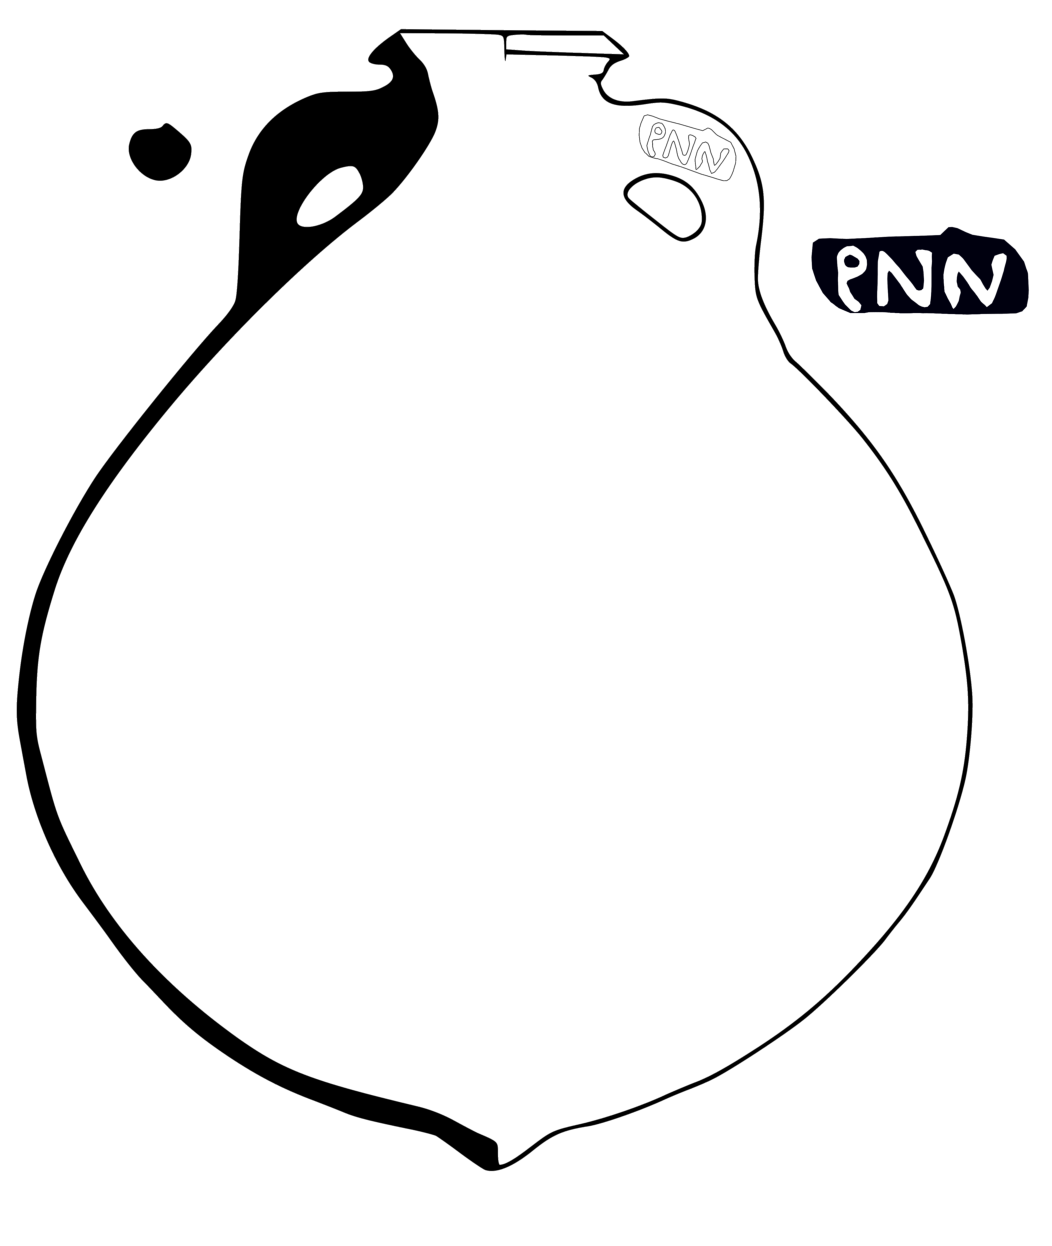
\includegraphics[scale=0.5]{figs/dressel20}
\caption{Dressel 20 were mostly marked with stamps of three letters called \textit{tria nomina}}
\label{amphora}
\end{figure} 

Frequently, they were mainly marked  in handles, but seldom in rims and body \citep{millet_anforas_1998}. 
The information of the stamps is shown in different forms and letter content and it seems that there was not a unique criterion. Stamps are mostly formed by a code of three letters and they can appear in abbreviated form or complete and they are known as \textit{Tria Nomina} \citep{berni_millet_amphora_1996}. Despite researchers identify stamps as identity marks, there is not a general consensus about the meaning of the stamps \citep{rodriguez_baetican_1998}. Alike most Dressel 20 containers were not stamped being difficult to determinate. 

They could be identified based on three premises: content (olive oil), context (amphora workshop) and subject (individuals involved). On the one hand, it seems that stamps could have been identified as the land owner of the olive groves \citep{rodriguez_economioleicola_1977}. On the other, they could belong to the owner of the making amphorae workshops or even a group of amphora workers \citep{berni_millet_epigrafianforica_2008}. In any case, the use of these stamps became in a good proxy to define somehow the system of working in the workshops. 

Nevertheless, some challenges remain under discussion such as how this production was organised and whether it is possible to distinguish production patterns in the olive oil trade. Our questions will be focused on the distribution of amphoric stamps. Did they follow a distribution pattern? Did stamps share the same workshop? Neither written records have been found that it could explain the economic role of \textit{Baetica} province in the Roman organisation. Indeed, archaeological evidence shows a highly specialised production with a long activity in this specific area with apparently few changes \citep{remesal_anforas_2004}. 


%\subsubsection{Jaccard distance}
%The dataset was analysed using a statistic method as Jaccard distance. This method allows to measure the dissimilarity by calculating the presence of sets (CITAR). In our case, Jaccard distance was used to compute the mutual presence of traits in the amphora stamps but it does not consider the number of absences. A comparison was done with the distance of the workshops to identify whether there was an association between stamps and spatial distance amongst workshops. 


\section{Method and Analysis}

The assumption of this study is analysing the effect of the production patterns between different centres. We are specially interested in identifying links between producers and consumption centres using amphoric stamps. To do that, we use the CEIPAC database to collect the stamps from different places. The CEIPAC dataset contains over 50.000 of epigraphy records found in amphorae, mostly from \textit{Monte Testaccio}. Therefore, this study proposes a robust baseline to explore the distribution of Baetican olive oil production by computing the spatial correlation between stamps. A way to analyse is to use a quantitative framework to measure the similarity between amphoric stamps. Here we use an ecological approach based on three steps: a) to detect similarities between stamp codes, b) to explore a potentially spatial correlation and c) to establish a correlation between similarity of stamps and spatial distance. 
%\xavi{no veo la parte evolutiva en el paper; por otra parte, si es relevante no la lanzaría aquí al vuelo; hace falta explicar por qué es necesaria, qué implica, etc.}

\subsection{Production centres: Baetica province}

We studied a dataset of 3798 stamps collected from different Dressel 20 amphora workshops in \textit{Baetica} province. The stamp database was compiled by CEIPAC group \citep{remesal_centro_2015} (see CEIPAC database here \url{http://romanopendata.eu}). However, approximately the 70 \% of stamps cannot be tested due to fragmentation or incomplete information. Consequently, we discard integrate the fragmented stamps in our dataset. We finally filtered a total sample of 987 stamps composed of 130 different stamps from 81 workshops. 


%3798 = base de datos sin limpiar
%3791 = base de datos limpiada con cleanstamp.py
%3787 = no sé a qué corresponde pero es archivo baetica.csv

From the database, we collected the site where stamps were found and the stamp code. We also created a new column with the area of the stamps. These areas, known as \textit{conventus}, were administrative centres for territorial organization in the Roman Empire. Dressel 20 stamps were found in three different \textit{conventus}: \textit{Hispalensis} (currently Seville, hereafter Hispalis), \textit{Cordubensis} (currently C\'ordoba, hereafter Corduba) and \textit{Astigi} (currently Écija, Sevilla, hereafter Astigi) \citep{rodriguez_economioleicola_1977,
chicdatos2001,berni_millet_epigrafianforica_2008} .

%\xavi{a ver, esto queda raro...si esto es una exploración de la base de datos entonces tiene que ir dentro de "Materials", así mientras vas comentando los sesgos y cosas generales de los datos (como soporte, pero no hace falta subsubsección "EDA")}

We calculated the frequency of distribution in amphora stamps with the aim to carry out an exploratory analysis (EDA) to know the distribution and the number of stamps per each centre.  

The frequency of stamps per workshop can be seen in Fig. \ref{stamps}. Most stamps are distributed in only one workshop whereas few workshops concentrate a high frequency of different amphoric stamps. The type of distribution is also frequent in amphora production where we observed a self-organized complex system pattern with a major concentration of the number of stamps in a few workshops \citep{bayesian_2018,coto-sarmiento_identifying_2018}.

%The type of distribution is also frequent in the Roman economy where we observed a self-organised complex system pattern typical of a free market 
%\xavi{quieres decir que esto es una power base? yo creo que no, no es tan bestia no? Yo lo matizaría}


\begin{figure}[htp]
	\centering
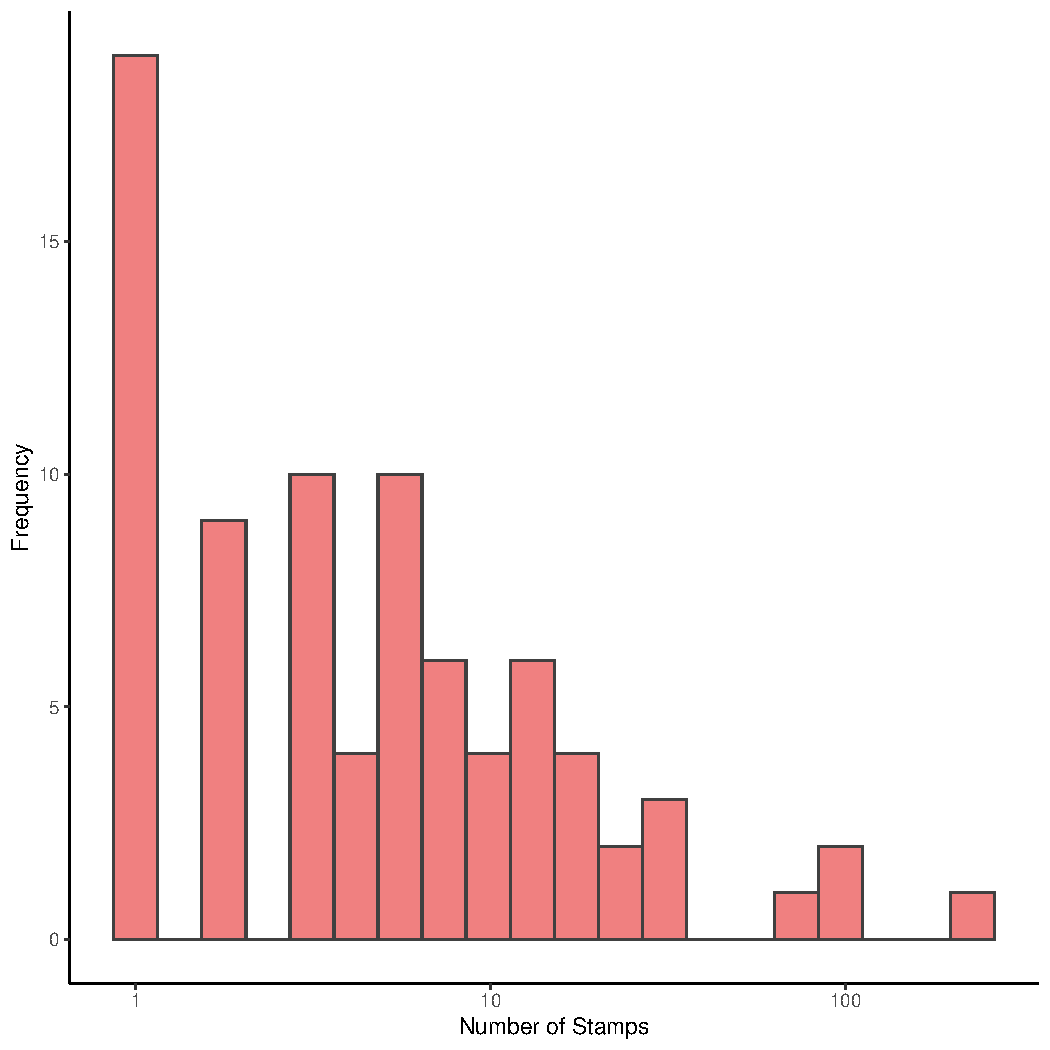
\includegraphics[width=\linewidth]{figs/frequencystamp.pdf}
\caption{Histogram with the number of stamps (X axis) and the frequency of distribution per workshop (Y axis). The distribution is widely diverse with most workshops concentrated one stamp}
\label{stamps}
\end{figure} 


The distribution of amphora stamps in different \textit{conventus} can be seen in Fig. \ref{frequency}. The majority of stamps found are concentrated in \textit{Hispalis} with 574 stamps while \textit{Corduba} and \textit{Astigi} with 267 and 146 stamps, respectively. Mostly, workshops show a homogeneity on the frequency of stamps except for both La Catria and Arva that exhibit a big amount of stamps with 29 different stamps. According to previous studies, those workshops became in most important centres of amphora production although they could have more intensely prospected than others. \citep{arva_1997}.
 
\begin{figure}[htp]
	\centering
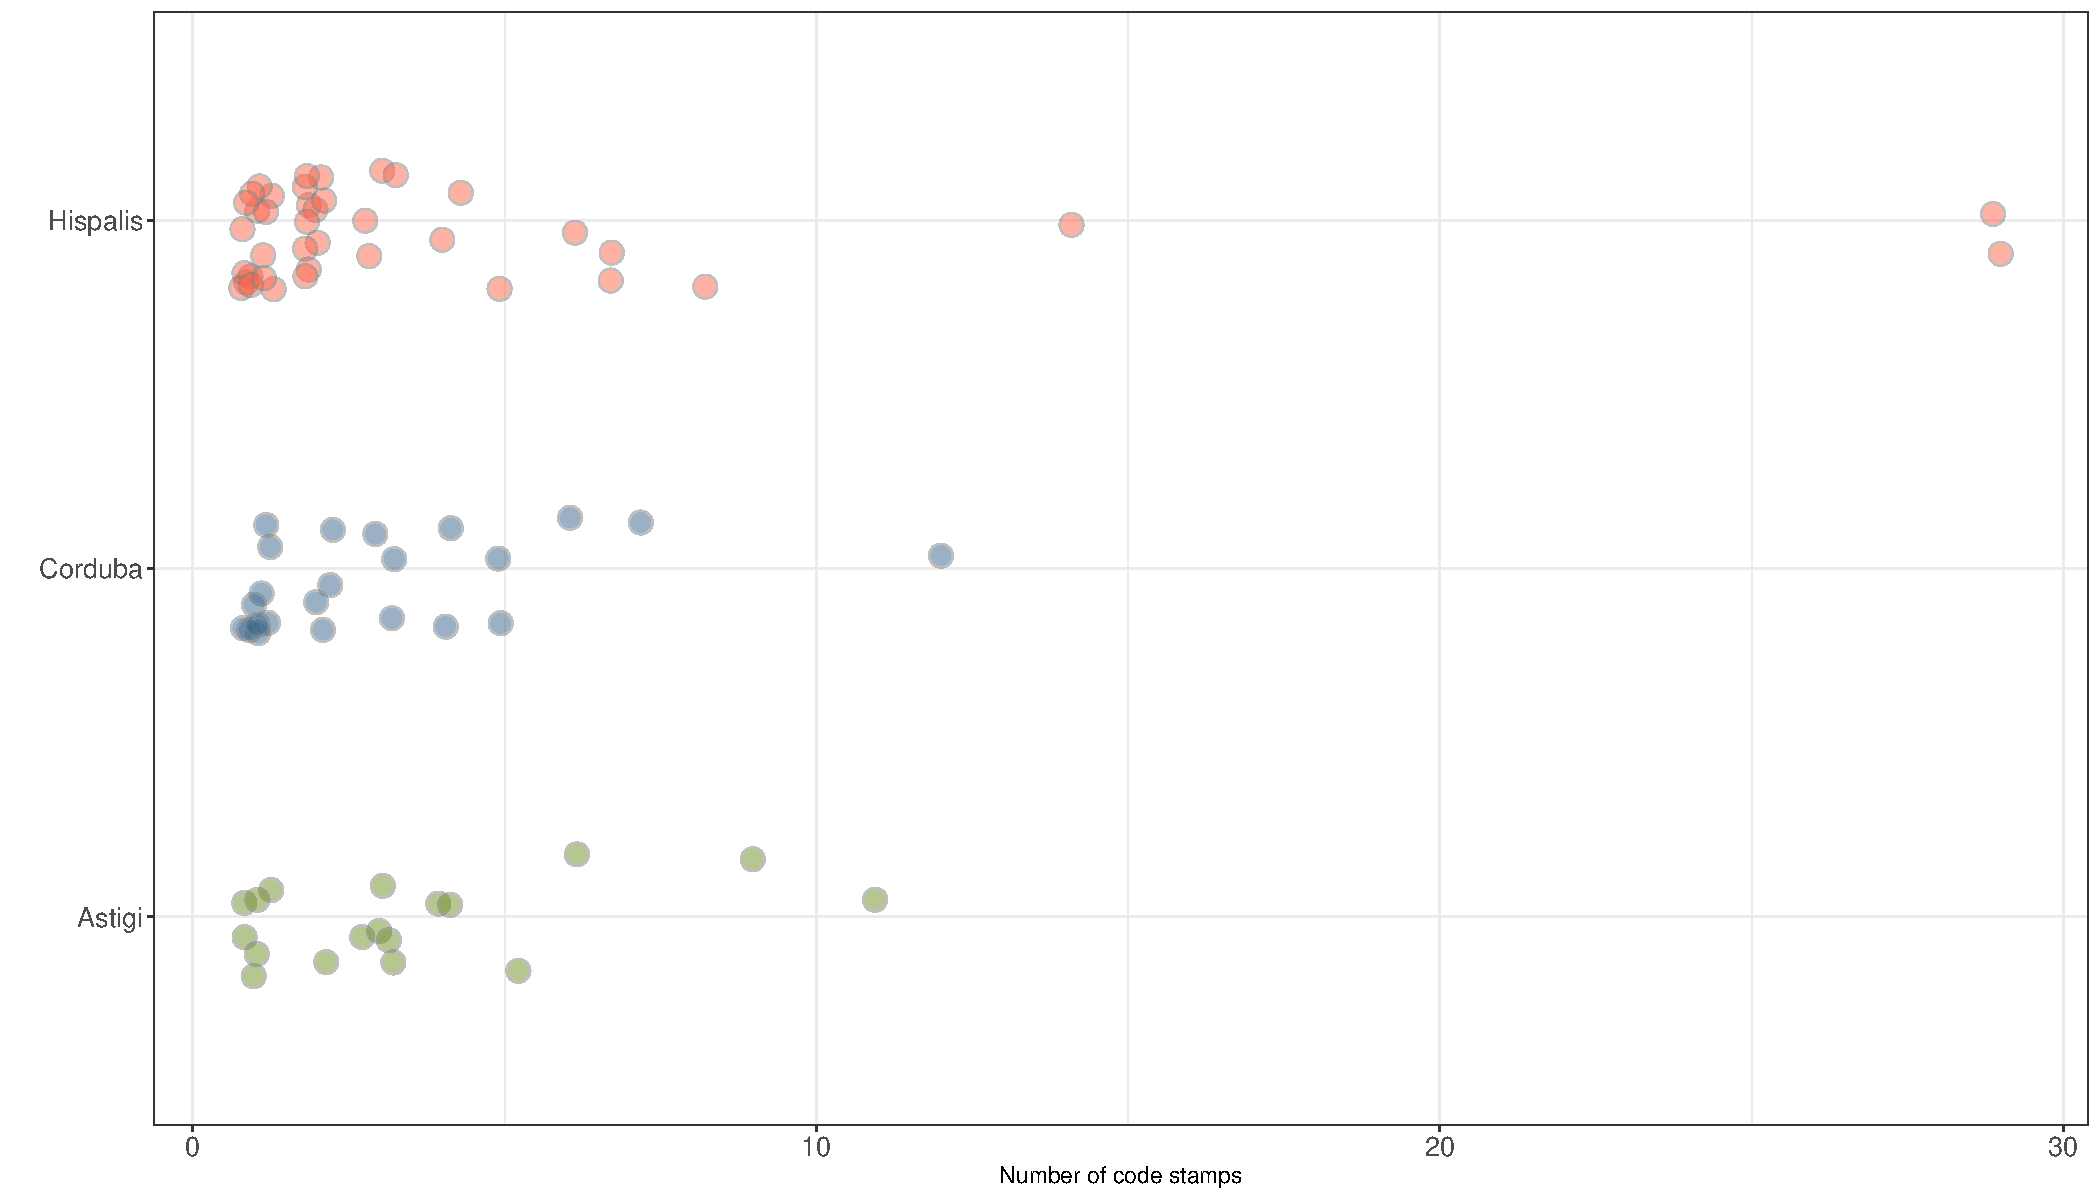
\includegraphics[width=\linewidth]{figs/frequency}
\caption{Distribution of the number of different code stamps (X axis) for each \textit{conventus} (Y axis). Colors are represented by areas divided into Hispalis (red), Astigi (green) and Corduba (blue)}
\label{frequency}
\end{figure} 


\subsection{Consumption centres: Britannia and Germania}


We analysed a dataset of 2219 stamps from different centres in \textit{Britannia}. 
%CITAR (Callender, 1965; Carreras Monfort y Funari,1998; Ayllón-Martı́ et al., 2018). 
The stamp database was also compiled by CEIPAC database. The database contained anomalies that were eliminated using the same criteria cited above. We finally selected the centres with more or equal than five stamps. As a result, we studied a total of 1765 stamps composed of 968 different stamps from 46 centres.
The centres located in \textit{Britannia} can be seen in Fig.\ref{britannia}.
 
\begin{figure}[htp]
	\centering
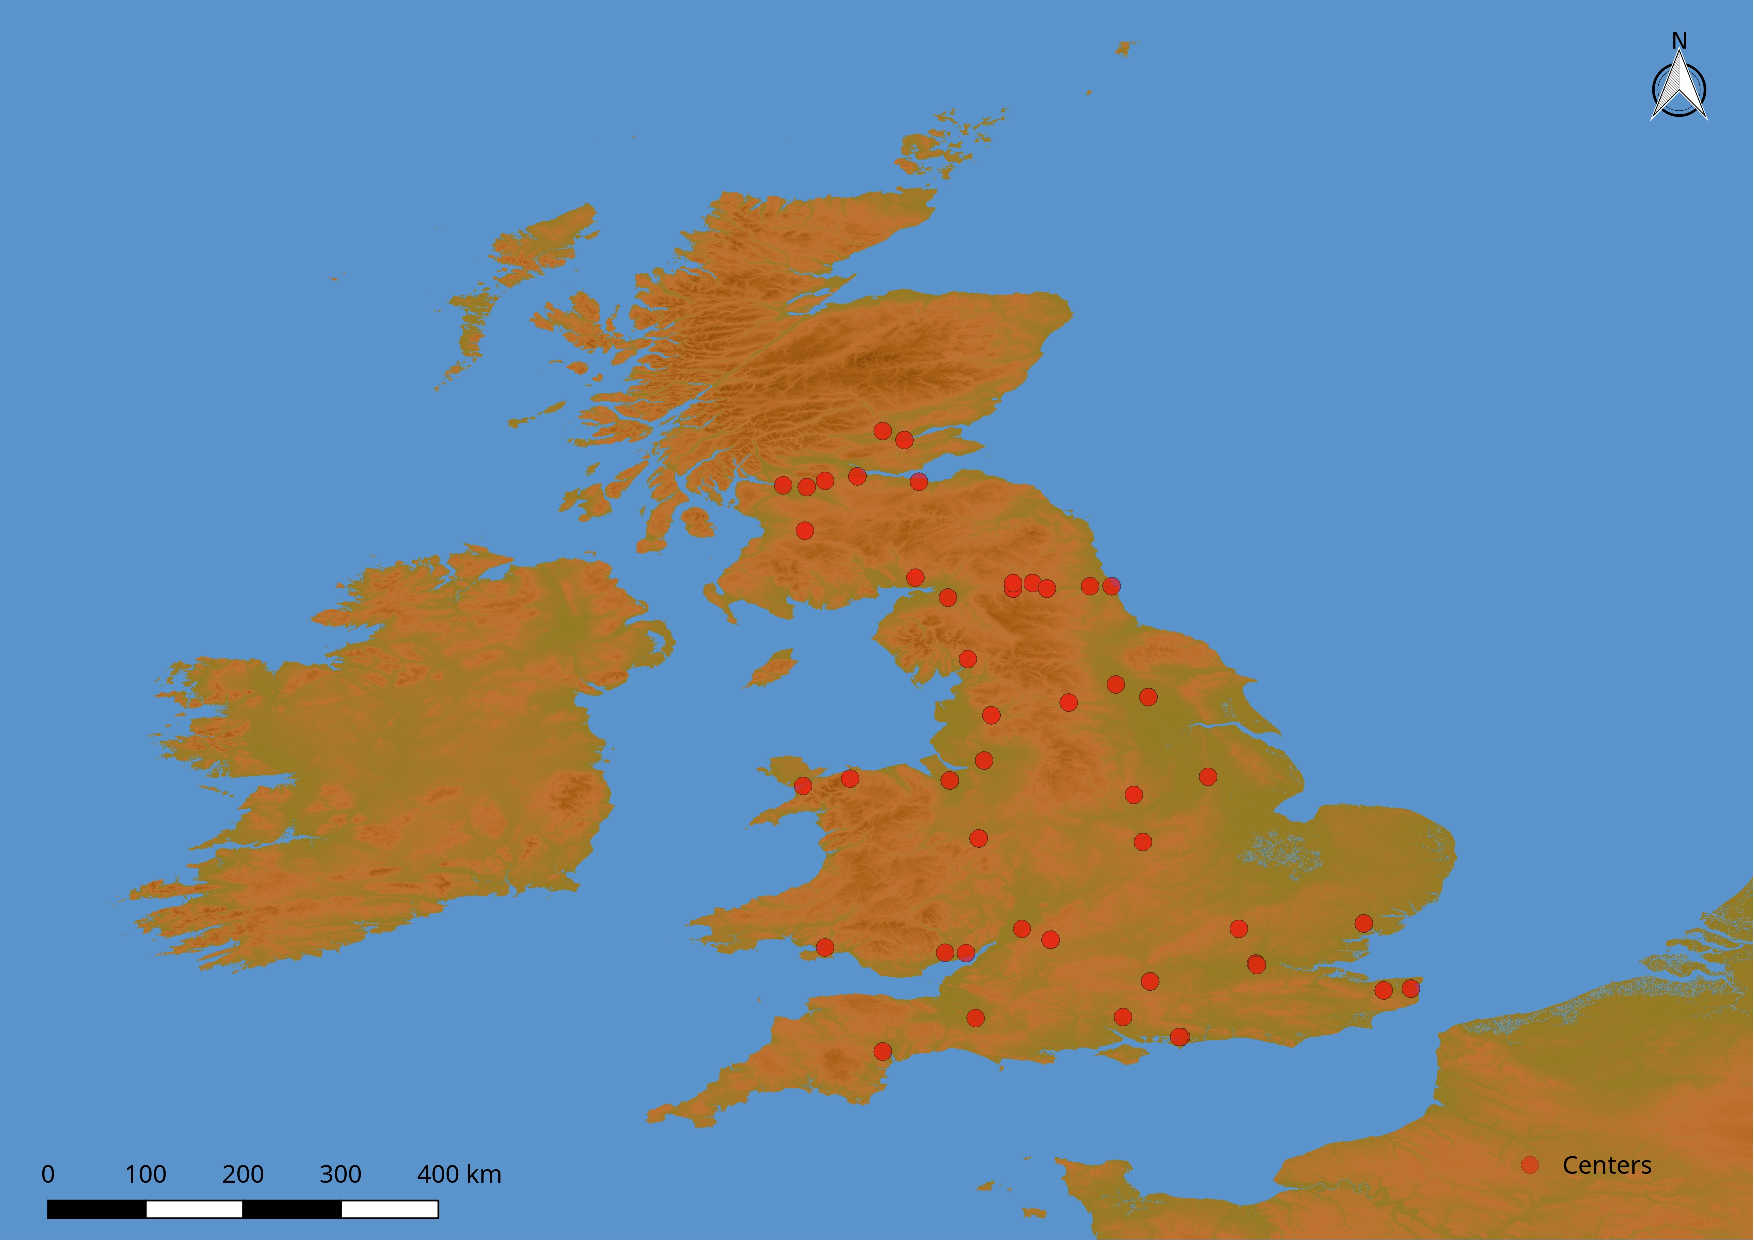
\includegraphics[width=\linewidth]{figs/britmap2.pdf}
\caption{Distribution of centres in \textit{Britannia}}
\label{britannia}
\end{figure} 


We analysed a dataset of 2052 stamps placed in \textit{Germania}. All the data was also compiled by CEIPAC database. We finally selected a total of 1621 stamps consisted of 850 different stamps from 46 sites (see Fig. \ref{germania}). As previously before, the centres were selected with more or equal than five stamps. 


\begin{figure}[htp]
	\centering
\includegraphics[width=\linewidth]{figs/germania5_2.pdf}
\caption{Distribution of the sites in \textit{Germania}. Most sites were located in limes during the Roman Empire}
\label{germania}
\end{figure}



\subsection{Measuring the dissimilarity in stamps}


%quizás habría que hablar también del filtrado de códigos que se hizo en python porque antes había 3783 stamps pero se filtró por el número de letras...
%\xavi{lo del filtrado lo puedes poner de supplementary information con referencia al antiquity}

The approach proposed here is based on the idea of measuring the similarity between amphora workshops by quantifying similar stamps. A measure of dissimilarity has been chosen to analyse the dataset. We use the statistical technique Morisita-Horn index \citep{morisita_measuring_1959, horn_measurement_1966}. This method was performed to measure the dissimilarity between different samples of sets. Generally, it describes the dissimilarity between the system of two communities based on the idea of inverse correlation between diversity and species \citep{magurran_why_1988}.

The formula can be described as follows \citep{magurran_measuring_2013}:

\begin{equation}
D(MH) = 1- \frac{2 \sum(a_{i} \cdot b_{i})}{(d_{a} + d_{b}) \cdot (N_{a} \cdot N_{b})}
\end{equation} \\

$d_{a}$ and $d_{b}$ are given by the following equation:

\begin{equation}
d_{a} = \frac{\sum a_{i}^{2}}{N_{a}^{2}} 
\end{equation} \\

where $N_{a}$ is the total number of stamps in workshop A; $N_{b}$ is the total number of stamps in workshop B; $a_{i}$ is the number of different stamps for workshop A and $b_{i}$ is the number of different stamps for workshop B.

Considering our dataset as a non-uniform sample, this method provides a useful tool to handle large samples with different sizes and diversity \citep{wolda_similarity_1981}. Morisita-Horn index can be expressed considering 0 as the total presence of similarity of stamps and 1 a total dissimilarity between stamps. In our case, it will be calculated the number of times that one stamp appears in an amphora workshop. This method allows to bear in mind a similar number of times for each repeated stamp per workshop. If two workshops have similar stamp codes, then the probability would be 0 whereas stamps codes are totally different when the results would be 1. 

\subsection{Hierarchical clustering}

Morisita-Horn index resulted in a numeric matrix of dissimilarities containing the distance value between the sites and the code stamps. The method was used to group sites with similar stamps codes. The matrix was then computed using hierarchical clustering. The algorithm was selected to cluster similar groups in order to analyse the relationship between groups of sites and the distribution of similar stamp codes. The results were visualised using a dendrogram to detect groups of sites sharing similar stamp codes.  


%\xavi{pero este es el único método que usas?}


\section{Results}

\subsection{Production centres: Baetica Province}

The analysis shows that amphoric stamps could be correlated with spatial distance. The correlation coefficients range from a minimum to a maximum. The dendrogram in Fig. \ref{dendro} was obtained with Morisita-Horn index. The dendrogram suggests that amphora workshops used different stamps for their production system. Nearby workshops show similarity on the stamps while most of them seem to display different stamps roles. Groups of workshops sharing similar stamps were not found in the cluster: the majority of stamp grouping was composed of no more than three workshops. Additionally, workshops that shared more similar amphoric stamps belonged to the same \textit{conventus} area, such as Picachos, Cerro de los Pesebres and El Castillejo. 

\begin{sidewaysfigure}[htp]
	\centering
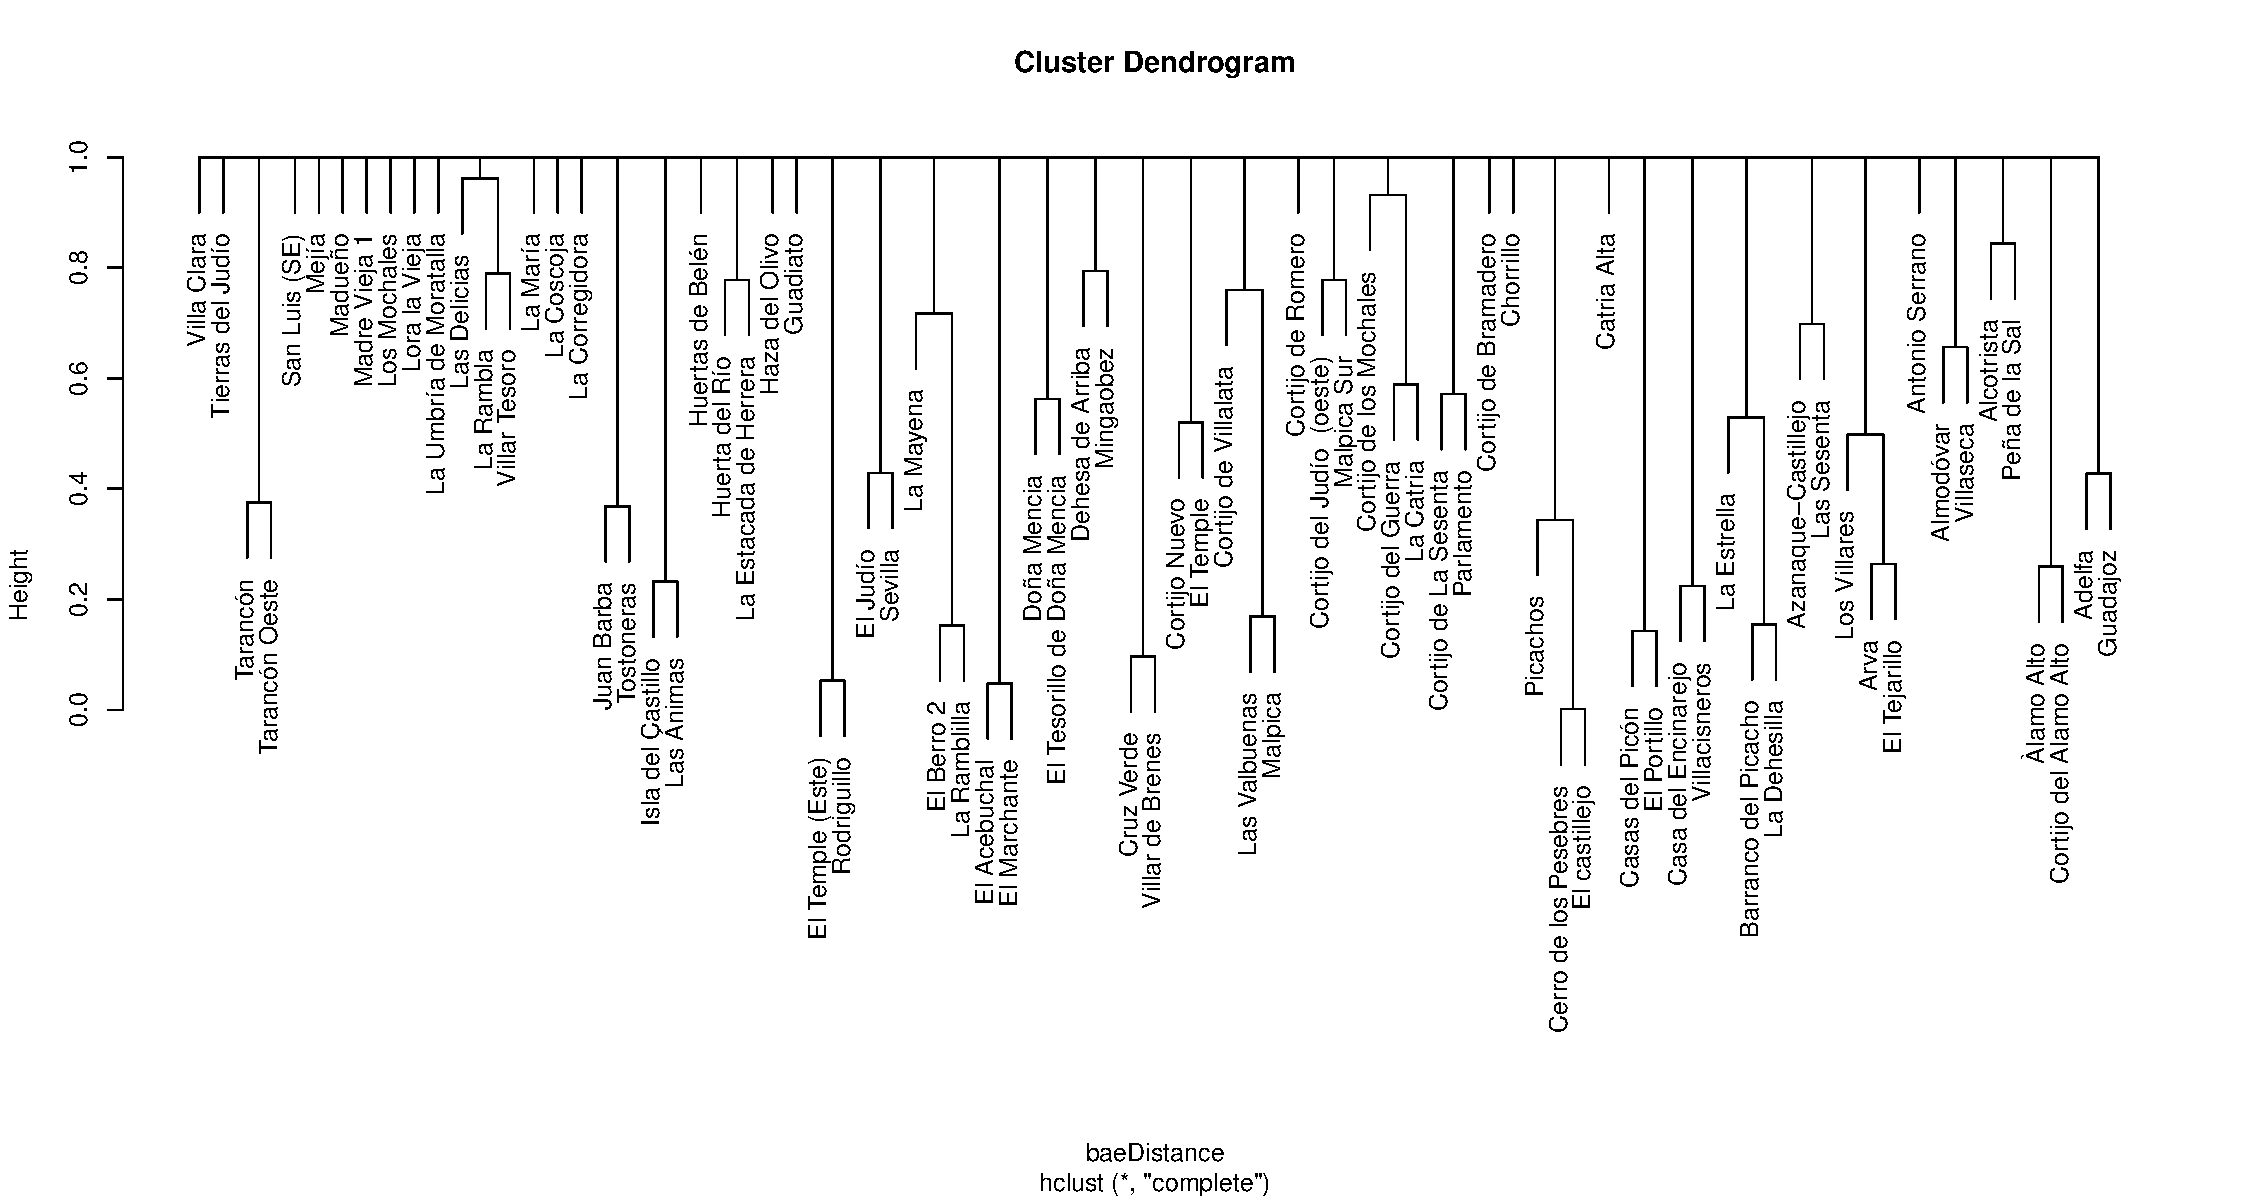
\includegraphics[width=\linewidth]{figs/dendro}
\caption{Dendrogram obtained by Morisita-Horn algorithm of different amphora workshops in \textit{Baetica} area. Colours are represented by areas divided into \textit{Hispalis} (red), \textit{Astigi} (green) and \textit{Corduba} (blue)}
\label{dendro}
\end{sidewaysfigure} 


\subsection{Reception centres: Britannia and Germania}


The results show a similarity with the results obtained in \textit{Baetica} province. However, the similarity is less pronounced as we observed in the dendrogram in Fig. \ref{britmap}

%\xavi{no tengo claro que le puedas decir correlación, porque eso es un valor específico entre 2 distribuciones numéricas. Te refieres a similaridad?}

\begin{sidewaysfigure}[htp]
	\centering
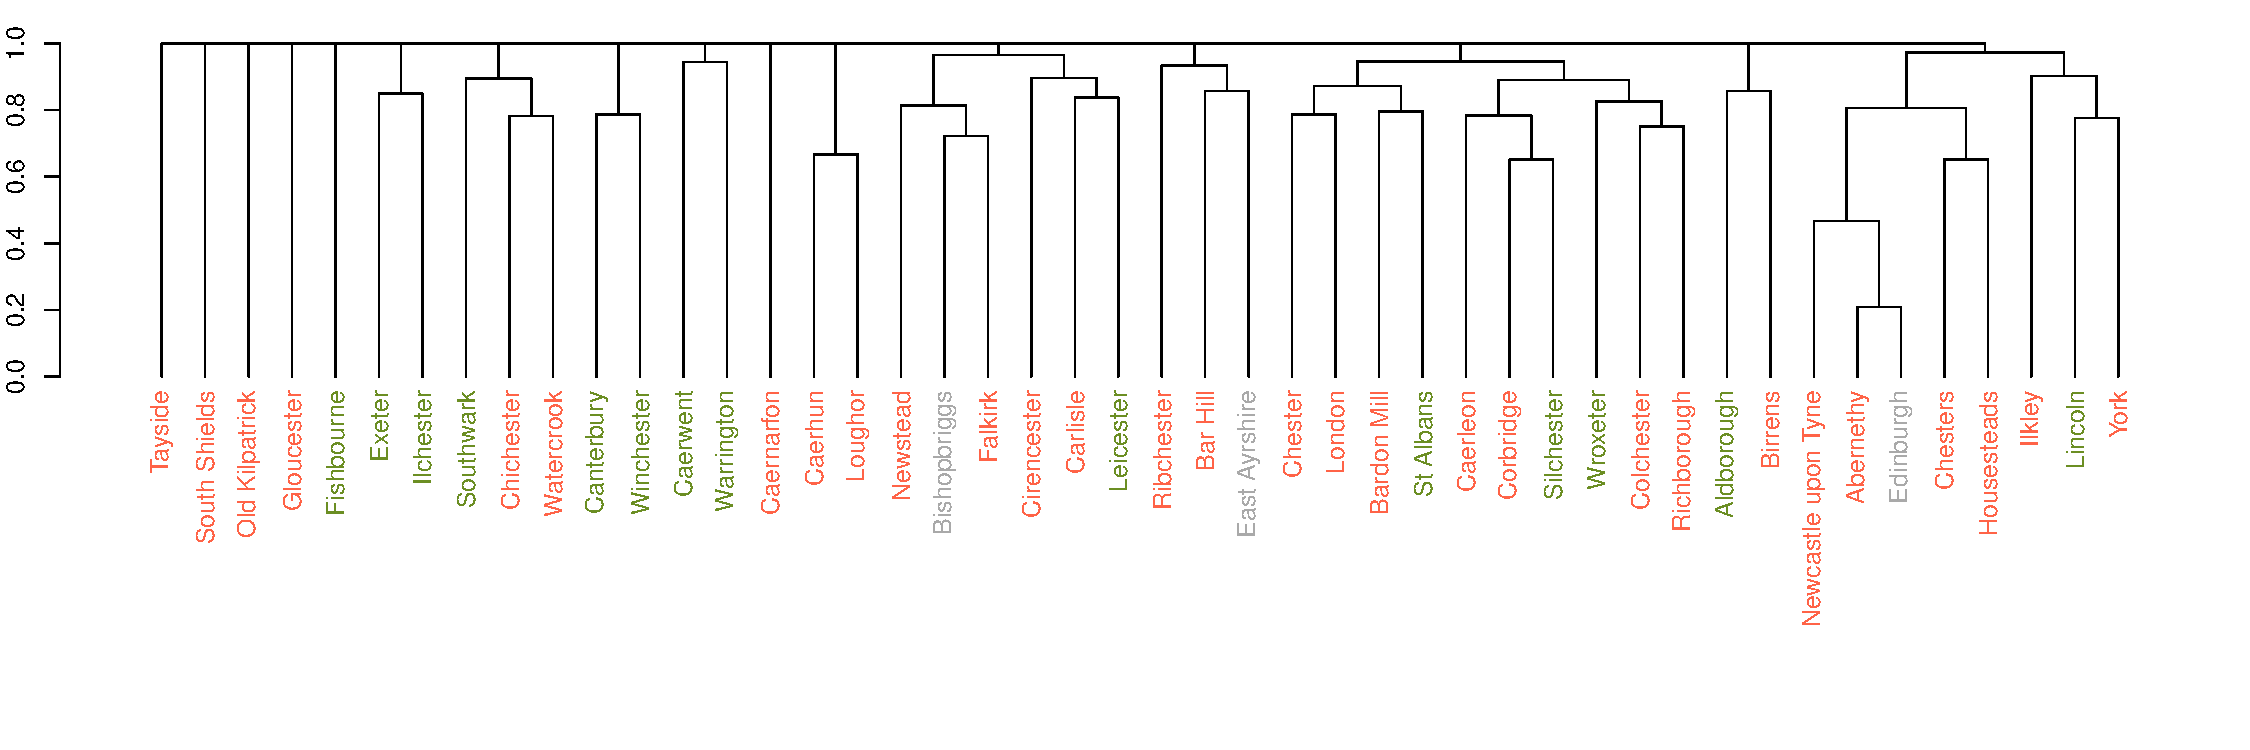
\includegraphics[width=\linewidth]{figs/dendrobrit5.pdf}
\caption{Dendrogram obtained by Morisita-Horn algorithm of different sites in \textit{Britannia}. Colours are represented by type of sites divided into military sites (red), civil sites (green) and no specific (grey)}
\label{britmap}
\end{sidewaysfigure}


A minor correlation can be explained by the fact that \textit{Britannia} spatial area is much wide than \textit{Baetica} where the centres were more concentrated.

Most military sites that showed greater similarity in the results were geographically close. We identified two factors in the results: 1) nearby sites tend to share similar stamps and 2) most sites have different stamps. 
By contrast, most sites did not show a strong similarity in stamp correlation. Neither we found a grouping of similar stamps in a specific place. In general, we did not observe any production pattern that indicates a clear organisation between production centres and reception centres. In other words, our results did not indicate the presence of a specific production center from \textit{Baetica} in \textit{Britannia} province. Rather, it seems that olive oil production was distributed by non-specific production centres. 


The similarity of stamps shows results less significant than \textit{Britannia} province as it can be seen in the dendrogram (Fig. \ref{germap}). 

\begin{sidewaysfigure}[htp]
	\centering
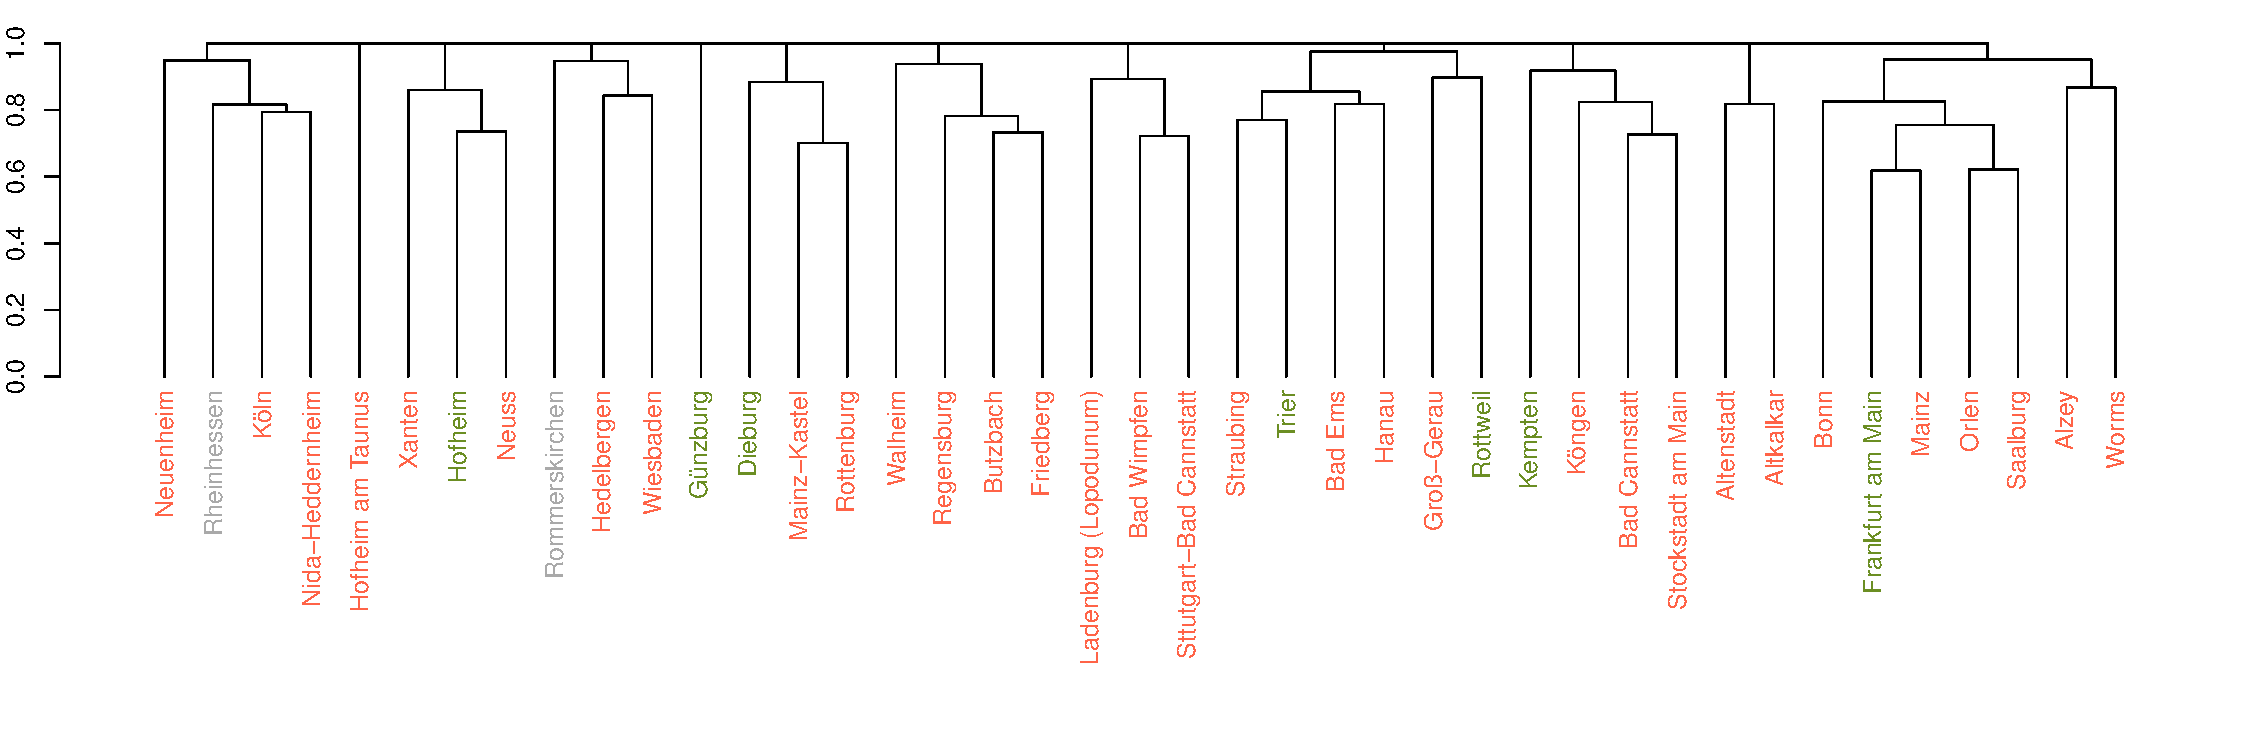
\includegraphics[width=\linewidth]{figs/dendroger5.pdf}
\caption{Dendrogram obtained by Morisita-Horn algorithm of different sites in \textit{Germania}. Colours are represented by types of sites divided into military sites (red), civil sites (green) and no specific (grey)}
\label{germap}
\end{sidewaysfigure}


The sites with more similarity in stamps were closely located in limes. In this case, most sites have different stamps which means that we did not detect any pattern. On the other hand, there seems to be a greater concentration of the seals in areas eminently militarised and close to the German limes. However, It is still no possibility to determine the existence of a defined pattern that reflects in more detail the route of this production in the area of the German limes.


\section{Discussion}


In this work, we aimed to analyse the distribution of the amphoric stamps in the organisation of the olive oil market both in the production and consumption areas. For this reason, an index of dissimilarity was used to detect differences between the distribution of the amphoric stamps and the spatial distance of producers and consumption centres. The general purpose was to explore if such differences found in the stamp codes could play an important role in the Roman market.  

\subsection{Production centres}

The analysis of the amphora workshops in Baetica province resulted in a significant correlation between spatial distance and the similarity of the amphoric stamps. 

The analysis suggests that there is  a connection between the same stamp code and nearby amphora workshops, excluding certain exceptions. Consequently, the majority of stamps are located in different amphora workshops and only similar stamps between closer amphora workshops were found. Indeed, our results show that most similar stamps were detected in the same \textit{conventus} area. This results can indicate a grouping of stamps with similar codes in the same \textit{conventus}. However, these stamps tend to share the same area of production but there is not a general relation between groups of amphora workshops and connection areas. In other words, we do not identify groups of more than three workshops or less sharing the same amphoric stamps as the dendrogram showed. In general, the majority of stamps were located in different amphora workshops. 


Our results indicate that the hypothesis about groups of amphora workshops sharing the same stamps seems do not match with the results of the analysis, even though there are similar stamps in closer workshops. Rather, it seems that each workshop was organised independently with different stamps. Those stamps detected in closer workshops do not move from other distant workshops. In other words, the stamps tend to remain in the same area and different stamps were located in a same amphora workshop. 

This could be defined by several factors. First, each workshop had a different organisation involved in the use of stamps and they were not used in other workshops. Second, stamp similarity in closer workshops could be linked to a spatial pattern. It is more probably than closer workshops tend to share more traits than distant workshops. While the role of the river was significant for the distribution of amphorae in consumption places, river connection amongst workshops does not seem to show relevancy for the distribution of stamps. Finally, the distribution of stamps could have shown some research bias. In some cases, workshops have been catalogued with different names in spite of belonging to the same workshops or being closer between each other. Additionally, most of the workshops were not widely excavated. 


\subsection{Consumption centres}

Both consumption centres showed a correlation between spatial distance and similarity in the amphoric stamps. In the case of\textit{Britannia}, the correlation was higher than \textit{Germania}.

In \textit{Britannia}, the majority of similarity stamps were mainly found in military centres. This could be also interpreted by a intense bias where military centres have been mostly excavated than civil centres. 

It is worth to mention that centres with a similarity correlation were located close to the Atlantic coast around the North Sea and the Celtic Sea. This could indicate that the Atlantic route could have played an essential role in transporting olive oil to the area of \textit{Britannia}, since in the places where there is greater similarity they are found in different strategic points near the sea.

This fact seems to concur with the latest research that suggest the idea of a more important Atlantic route that would connect the provinces militarised\citep{remesal_annona_1986,
remesal_provincial_2008,
carreras_atlantic_2012,
morillo_hispania_2016,rubio-campillo_provincias_2018}.

Therefore, most part of the centres where similar stamps are shared can correspond to eminently military areas, which may mean that the transport could reach the military areas from the beginning and then be distributed by land routes along with other civil areas \citep{carreras_britannia_1998,
ayllon_olive_2018}.

In \textit{Germania}, the results followed the same pattern as \textit{Britannia} but with a minor correlation as we can observe in the dendrogram. The areas mostly militarised share similar stamps than civil areas. However, we do not detect a concrete pattern regarding the distribution of the stamps in the German limes \citep{xanten2018}. 

It is worth to mention that it was not detected a robust model of organisation in both cases with regard to the distribution of stamps in consumption centres. This means
that it is unknown whether certain production centres went to one province or another or, at the
less, that it can be clearly reflected in the data with a greater similarity in the amphoric stamps. Thus, production centres could have distributed randomly olive oil both \textit{Britannia} and \textit{Germania}. We do not detect production centres dedicated to the distribution of olive oil in a certain province. 

In general, we observed a distribution of the stamps to military stamps. By contrast, judging by the results obtained, there does not seem to be a specific pattern in terms of geographical distribution. Nor it was detected consumption areas where stamps are specified from an amphora workshop. 


\section{Conclusion}


The results of the case study could be interpreted by several reasons. On the one hand, the use of these amphoric stamps could have been exclusively running by the owner or owners of the workshop to distinguish the amphora workshop. This hypothesis would explain the fact that we do not find similar stamps in different workshops; however, we found different amphora stamps in the same workshops that they would be barely difficult to assign different owners.

On the other hand, the existence of different stamps in the same workshop but which are only repeated in very close places it would imply some kind of organisation from within workshop affecting the closest centres. This could be explained such as batch systematic organisation between potters \citep{juanmorostesis}. 
This method allowed to potters organise the production with the batch stamping for the posterior commercialisation.

Considering that Dressel 20 was not marked in most cases, some researchers point out that potters marked amphorae to prepare and distribute the commodity to be shipped \citep{berni_millet_epigrafianforica_2008}. This method would be used as an identifier to count the number of amphorae of a branch \citep{juanmorostesis}. This organisation could also have served to identify different groups of potters working in the same amphora workshop. Potters could have marked the amphorae to distinguish different groups working in parallel \citep{li_crossbows_2014}. This fact would explain wherefore why we detect different stamps in the same workshop. In any case, we do not have enough archaeological evidence that can validate the interpretations presented here and our results are certainly valid only with the context of our case study. 

As a summary, this method presented here provides a potential tool to understand mechanisms of production based on the similarity of artefacts. This work has identified differences in the case of the amphoric production within the Roman Empire. Accordingly, the results have highlighted for the interpretation of the complex economic processes connected with the archaeological evidence. 


\section{Acknowledgements}

The research was funded by European Research Council Advanced Grant EPNet (340828). We are grateful to Simon Carrignon, Juan Moros and Ignacio Morer for their useful suggestions.  
All data has been analysed and conducted in R program version 3.2.4, using the packages \textit{vegan} \citep{oksanen_vegan_2007}, \textit{ggplot2} \citep{ggplot2:_2016}. Source and code are available at \maria{incluir github}. 


\section{References}

%\bibliography{bibliotex}
\bibliography{bibtesis}



\end{document}
